% !TEX TS-program = pdflatex
% !TEX encoding = UTF-8 Unicode

\documentclass[11pt]{report} % use larger type; default would be 10pt

\usepackage[utf8]{inputenc} % set input encoding (not needed with XeLaTeX)

%%% Examples of Article customizations
% These packages are optional, depending whether you want the features they provide.
% See the LaTeX Companion or other references for full information.

%%% PAGE DIMENSIONS
\usepackage{geometry} % to change the page dimensions
\geometry{a4paper} % or letterpaper (US) or a5paper or....
% \geometry{margin=2in} % for example, change the margins to 2 inches all round
% \geometry{landscape} % set up the page for landscape
%   read geometry.pdf for detailed page layout information

\usepackage{graphicx} % support the \includegraphics command and options

% \usepackage[parfill]{parskip} % Activate to begin paragraphs with an empty line rather than an indent

%%% PACKAGES
\usepackage{listings}
\usepackage{lipsum}
\usepackage{courier}

\lstset{basicstyle=\footnotesize\ttfamily,breaklines=true}
\lstset{framextopmargin=50pt}

\usepackage{booktabs} % for much better looking tables
\usepackage{array} % for better arrays (eg matrices) in maths
\usepackage{paralist} % very flexible & customisable lists (eg. itemize/itemize, etc.)
\usepackage{verbatim} % adds environment for commenting out blocks of text & for better verbatim
\usepackage{subfig} % make it possible to include more than one captioned figure/table in a single float
% These packages are all incorporated in the memoir class to one degree or another...

%%% HEADERS & FOOTERS
\usepackage{fancyhdr} % This should be set AFTER setting up the page geometry
\pagestyle{fancy} % options: empty , plain , fancy
\renewcommand{\headrulewidth}{0pt} % customise the layout...
\lhead{}\chead{Plugin Architecture Diagrams}\rhead{}
\lfoot{}\cfoot{\thepage}\rfoot{}

%%% SECTION TITLE APPEARANCE
\usepackage{sectsty}
\allsectionsfont{\sffamily\mdseries\upshape} % (See the fntguide.pdf for font help)
% (This matches ConTeXt defaults)

%%% ToC (table of contents) APPEARANCE
\usepackage[nottoc,notlof,notlot]{tocbibind} % Put the bibliography in the ToC
\usepackage[titles,subfigure]{tocloft} % Alter the style of the Table of Contents
\usepackage{graphicx}

\renewcommand{\cftsecfont}{\rmfamily\mdseries\upshape}
\renewcommand{\cftsecpagefont}{\rmfamily\mdseries\upshape} % No bold!

%%% END Article customizations

%%% The "real" document content comes below...

\title{Software Engineering Project - Links \\Plugin Architecture and Plugin Creation Guide}
\author{Abhijith Madhav, Arjun S Bharadwaj}
%\date{} % Activate to display a given date or no date (if empty),
         % otherwise the current date is printed 

\begin{document}
\maketitle
\section*{Plugin architecture diagram}
Below is the plugin architecture diagram of ``Links''.
\begin{figure}[h]
\centering
        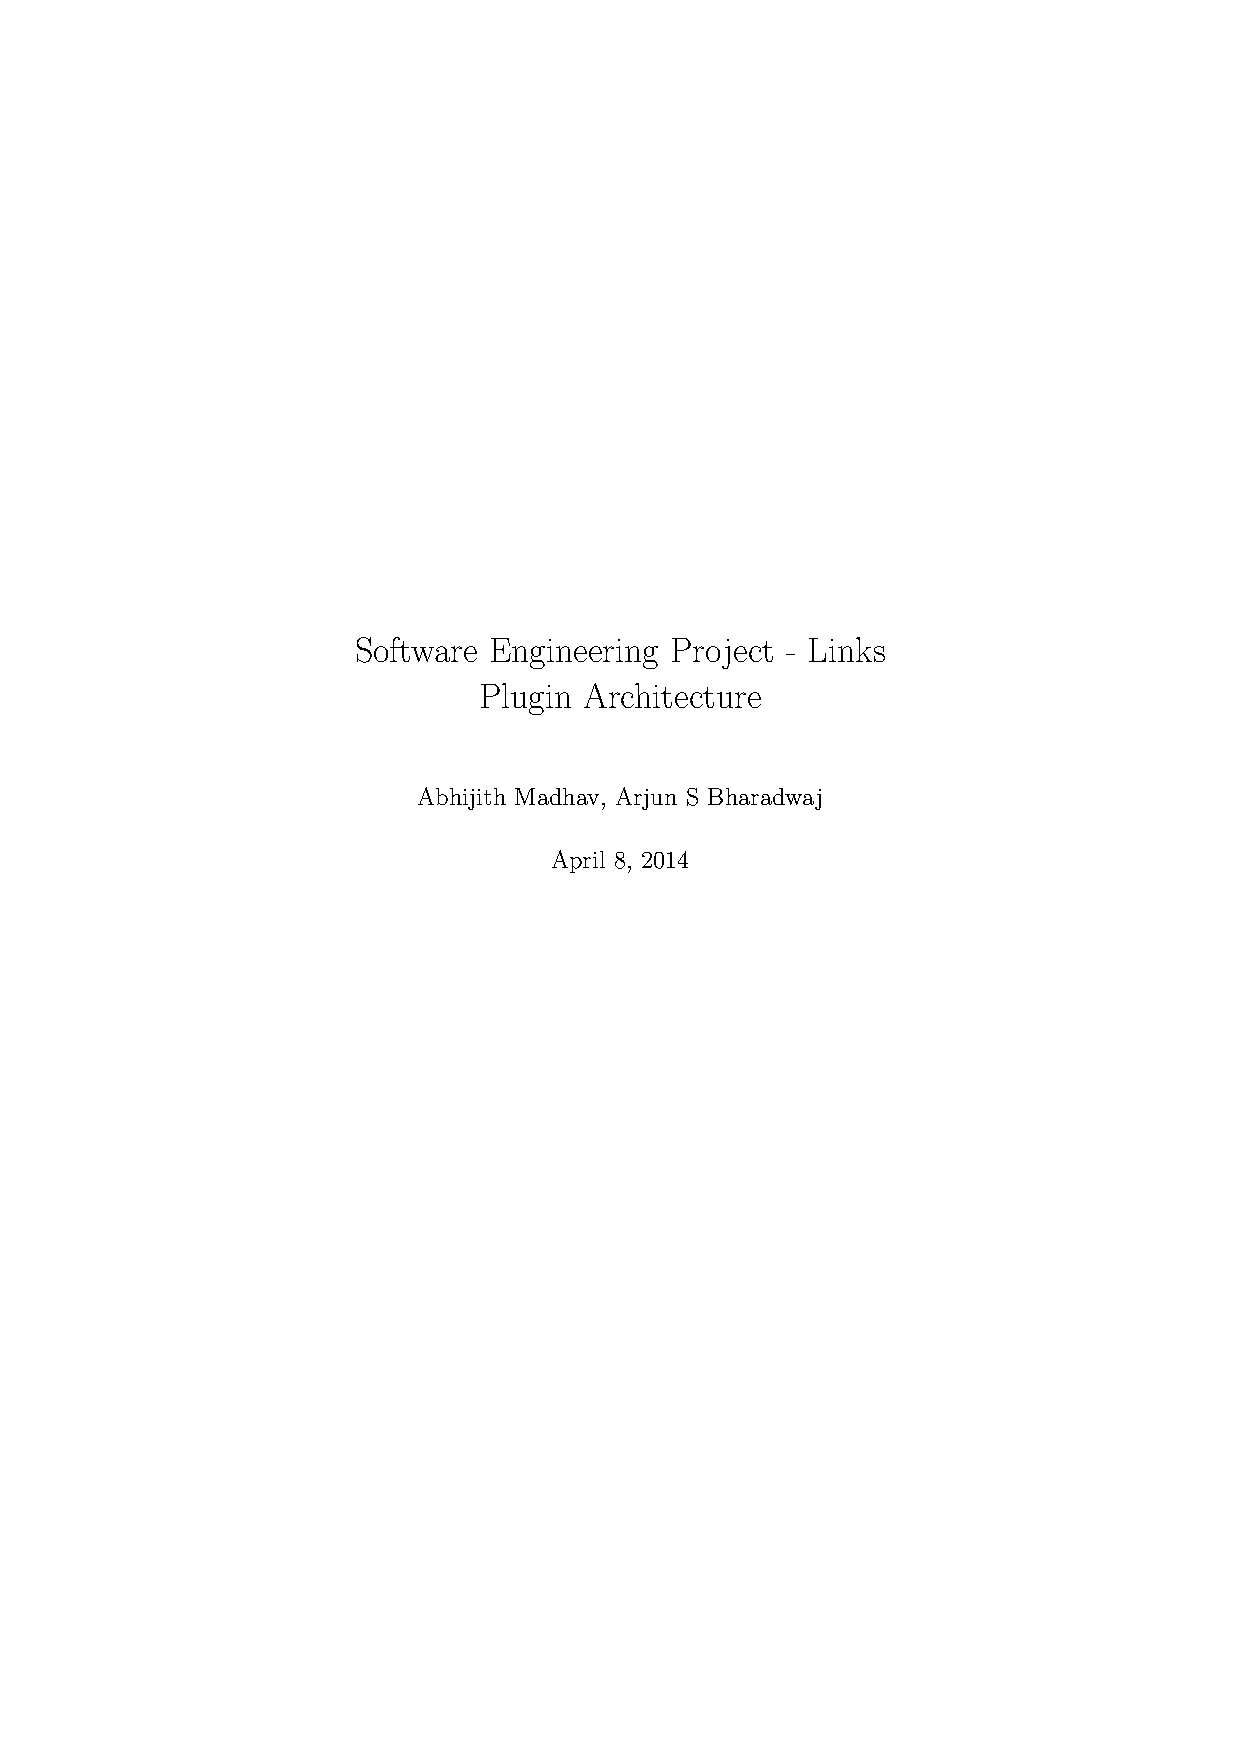
\includegraphics[width=\textwidth]{PluginArchitecture}
    \caption{{Links - Plugin Architecture Diagram}.}
    \label{fig:Plugin Architecture Diagram}
\end{figure}


These are the components of the Plugin Architecture.
\begin{enumerate}

\item
	Configuration File: This file will consist of all the plugins that are enabled in the system.
\item
	Plugin Manager: The Plugin Manager will lookup the configuration file and will enable/disale the plugins.
\item
	Share Plugin: This plugin will help to share the links on various platforms like Email, Twitter and Facebook.
\end{enumerate}

\section*{Plugin creation guide in Rails}
A plugin is a fully functional rails app. It can be made mountable so that it could be used only with the main app.

\begin{enumerate}
	\item
	Create a new rails project in Rails. 
	\begin{lstlisting}
Ex: rails new links
	\end{lstlisting}
	Here, a project called links is created.

	\item
	Create a plugin project and make it mountable.
	\begin{lstlisting}
Ex: rails plugin new share --mountable
	\end{lstlisting}
	Here, a plugin called share is created.

	\item
	Add the dependency gem in the main project in ``Gemfile''.
	\begin{lstlisting}
gem 'share', path: "../share"
	\end{lstlisting}
	Here, a gem called ``/share'' is added as dependency in the main project and ``bundle install'' is executed in the main project. The path is relative here. If the Engine is published as Gem, the gem location can be given too.
		
	\item
	Add a mount point in the main project in ``routes.rb'' file.
	\begin{lstlisting}
mount Share::Engine, :at => "/share"
	\end{lstlisting}
	Here, a mount point at ``/share'' is created. So all the controllers of share plugin can be access via ``/share'' path.
	
\end{enumerate}

\end{document}
